% DataSynth Executive Overview
% Compile with: pdflatex datasynth-executive-overview.tex (run twice for TOC)
\documentclass[11pt,a4paper]{article}

% ── Packages ──────────────────────────────────────────────────────────────────
\usepackage[utf8]{inputenc}
\usepackage[T1]{fontenc}
\usepackage{lmodern}
\usepackage[margin=2.4cm]{geometry}
\usepackage{graphicx}
\usepackage{xcolor}
\usepackage{titlesec}
\usepackage{enumitem}
\usepackage{booktabs}
\usepackage{tabularx}
\usepackage{multirow}
\usepackage{fancyhdr}
\usepackage{hyperref}
% fontawesome5 removed — using text symbols instead
\usepackage{tcolorbox}
\usepackage{needspace}
\usepackage{tikz}
\usepackage{pgfplots}
\usepackage{amssymb}
\pgfplotsset{compat=1.18}
\usetikzlibrary{arrows.meta, positioning, calc, shapes.geometric, backgrounds, fit}

% ── Colours ───────────────────────────────────────────────────────────────────
\definecolor{brand}{HTML}{1A2744}      % Deep navy
\definecolor{accent}{HTML}{2E86AB}     % Teal blue
\definecolor{highlight}{HTML}{F18F01}  % Amber
\definecolor{success}{HTML}{2D936C}    % Green
\definecolor{lightbg}{HTML}{F5F7FA}    % Light background
\definecolor{midgray}{HTML}{6C757D}    % Muted text

% ── Heading styles ────────────────────────────────────────────────────────────
\titleformat{\section}
  {\Large\bfseries\color{brand}}
  {\thesection}{1em}{}[\vspace{-0.4em}\textcolor{accent}{\rule{\textwidth}{1.2pt}}]

\titleformat{\subsection}
  {\large\bfseries\color{brand}}
  {\thesubsection}{0.8em}{}

\titleformat{\subsubsection}
  {\normalsize\bfseries\color{accent}}
  {\thesubsubsection}{0.6em}{}

% ── Header / Footer ──────────────────────────────────────────────────────────
\pagestyle{fancy}
\fancyhf{}
\renewcommand{\headrulewidth}{0.4pt}
\fancyhead[L]{\small\textcolor{midgray}{DataSynth --- Executive Overview}}
\fancyhead[R]{\small\textcolor{midgray}{v0.9.3}}
\fancyfoot[C]{\small\textcolor{midgray}{\thepage}}

% ── Custom boxes ──────────────────────────────────────────────────────────────
\tcbset{
  keybox/.style={
    colback=lightbg, colframe=accent, boxrule=0.6pt,
    arc=3pt, left=8pt, right=8pt, top=6pt, bottom=6pt,
    fonttitle=\bfseries\color{brand}, title=#1
  },
  statbox/.style={
    colback=white, colframe=brand, boxrule=0.8pt,
    arc=4pt, left=6pt, right=6pt, top=4pt, bottom=4pt,
    width=0.30\textwidth
  }
}

% ── Hyperref setup ────────────────────────────────────────────────────────────
\hypersetup{
  colorlinks=true,
  linkcolor=brand,
  urlcolor=accent,
  citecolor=brand,
  pdftitle={DataSynth -- Enterprise Synthetic Data Platform},
  pdfauthor={DataSynth},
  pdfsubject={Executive Overview},
}

% ══════════════════════════════════════════════════════════════════════════════
\begin{document}

% ── Title page ────────────────────────────────────────────────────────────────
\begin{titlepage}
\begin{tikzpicture}[remember picture, overlay]
  % Background gradient bar
  \fill[brand] (current page.north west) rectangle
    ([yshift=-9cm]current page.north east);
  % Accent stripe
  \fill[accent] ([yshift=-9cm]current page.north west) rectangle
    ([yshift=-9.4cm]current page.north east);
  % Decorative dots
  \foreach \x in {0.5,1.0,...,5.0} {
    \foreach \y in {0.5,1.0,...,3.0} {
      \fill[white, opacity=0.04] ([xshift=\x cm, yshift=-\y cm]current page.north west)
        circle (1.5pt);
    }
  }
\end{tikzpicture}

\vspace*{1.5cm}
\begin{flushleft}
  {\fontsize{38}{44}\selectfont\bfseries\textcolor{white}{DataSynth}}\\[0.5em]
  {\fontsize{16}{20}\selectfont\textcolor{white!85}{Enterprise Synthetic Data Platform}}\\[0.3em]
  {\large\textcolor{white!65}{High-Performance Generation for Accounting, Audit \& ML}}\\[0.3em]
  {\normalsize\textcolor{white!50}{Rust core \textbullet{} Python 1.3 \textbullet{} REST/gRPC API \textbullet{} Desktop UI \textbullet{} Helm/Docker}}
\end{flushleft}

\vspace{5.5cm}

\begin{flushleft}
  \textcolor{midgray}{\large Executive Overview}\\[0.8em]
  {\Large\textcolor{brand}{\textbf{Version 0.8.0}}}\\[1.5em]
  \textcolor{midgray}{%
    Deterministic, privacy-preserving synthetic data generation\\
    for enterprise finance, compliance testing, and machine learning.%
  }
\end{flushleft}

\vfill
\begin{flushleft}
  \textcolor{midgray}{\small
    Built with Rust \& Python \textbullet{} 15 modular crates \textbullet{} 100\,K+ entries/sec\\[4pt]
    Open-source (Apache-2.0) \textbullet{} Commercial license available\\[4pt]
    \textbf{Contact:} \href{mailto:michael.ivertowski@ch.ey.com}{michael.ivertowski@ch.ey.com}
  }
\end{flushleft}
\end{titlepage}

% ── Table of Contents ─────────────────────────────────────────────────────────
\tableofcontents
\newpage

% ══════════════════════════════════════════════════════════════════════════════
\section{Executive Summary}

DataSynth is a high-performance synthetic data platform purpose-built for
enterprise accounting, audit analytics, and machine learning. Written in Rust
for maximum throughput and memory safety --- with a full Python wrapper for
data-science workflows --- it generates realistic, internally coherent
financial data that satisfies the statistical and structural properties of
real-world enterprise resource planning (ERP) systems.

\begin{tcolorbox}[keybox={Why DataSynth?}]
\begin{itemize}[leftmargin=1.2em, itemsep=3pt]
  \item \textbf{No real data required} --- eliminates privacy, regulatory, and
        procurement barriers to analytics development.
  \item \textbf{Full auditability} --- deterministic, seeded generation means
        every dataset is perfectly reproducible.
  \item \textbf{ML-ready from day one} --- ground-truth labels for fraud,
        anomalies, and data quality ship alongside every record.
  \item \textbf{Domain depth} --- covers the full accounting lifecycle:
        journal entries, document flows, subledgers, FX, intercompany,
        period close, and banking/AML.
  \item \textbf{Empirically grounded} --- statistical distributions for
        journal entry line items, amount patterns, and temporal volumes are
        calibrated against empirical research conducted on real-world
        enterprise datasets, ensuring synthetic output mirrors the
        structural properties of production ERP data.
\end{itemize}
\end{tcolorbox}

\subsection{At a Glance}

\vspace{0.6em}
\begin{center}
\begin{tabular}{@{}c@{\hspace{1.8em}}c@{\hspace{1.8em}}c@{}}
% Row 1
\begin{tcolorbox}[statbox, width=4.8cm]
  \centering
  {\fontsize{26}{30}\selectfont\bfseries\textcolor{accent}{100\,K+}}\\[3pt]
  {\small entries/sec (single thread)}
\end{tcolorbox} &
\begin{tcolorbox}[statbox, width=4.8cm]
  \centering
  {\fontsize{26}{30}\selectfont\bfseries\textcolor{accent}{60+}}\\[3pt]
  {\small ACFE-aligned fraud schemes}
\end{tcolorbox} &
\begin{tcolorbox}[statbox, width=4.8cm]
  \centering
  {\fontsize{26}{30}\selectfont\bfseries\textcolor{accent}{10}}\\[3pt]
  {\small industry presets}
\end{tcolorbox} \\[0.8em]
% Row 2
\begin{tcolorbox}[statbox, width=4.8cm]
  \centering
  {\fontsize{26}{30}\selectfont\bfseries\textcolor{accent}{15}}\\[3pt]
  {\small modular Rust crates}
\end{tcolorbox} &
\begin{tcolorbox}[statbox, width=4.8cm]
  \centering
  {\fontsize{26}{30}\selectfont\bfseries\textcolor{accent}{50+}}\\[3pt]
  {\small red flag patterns}
\end{tcolorbox} &
\begin{tcolorbox}[statbox, width=4.8cm]
  \centering
  {\fontsize{26}{30}\selectfont\bfseries\textcolor{accent}{4}}\\[3pt]
  {\small privacy levels}
\end{tcolorbox}
\end{tabular}
\end{center}

% ══════════════════════════════════════════════════════════════════════════════
\newpage
\section{Platform Capabilities}

\subsection{Enterprise Accounting Simulation}

DataSynth generates a complete, internally consistent accounting universe:

\vspace{0.4em}
\noindent
\renewcommand{\arraystretch}{1.25}
\begin{tabularx}{\textwidth}{>{\bfseries\color{brand}}l X}
\toprule
\textbf{Domain} & \textbf{Capabilities} \\
\midrule
Journal Entries &
  Balanced debits/credits, Benford-compliant amounts, configurable line-item
  distributions, SAP ACDOCA format export. \\
Master Data &
  Vendors, customers, materials, fixed assets, employees with hierarchies,
  payment terms, credit ratings, and intercompany flags. \\
Document Flows &
  Full Procure-to-Pay (PO\,$\to$\,GR\,$\to$\,Invoice\,$\to$\,Payment) and
  Order-to-Cash (SO\,$\to$\,Delivery\,$\to$\,Invoice\,$\to$\,Receipt) with
  three-way match validation and contract price enforcement. \\
Intercompany &
  Matched IC journal entry pairs, transfer pricing (Cost-Plus, Resale-Minus,
  CUP), and consolidation elimination entries. \\
Subledgers &
  AR/AP open items and aging, fixed asset register with IRS MACRS depreciation
  tables (3--20\,yr recovery periods), inventory positions and movements,
  GL-to-subledger reconciliation. \\
FX \& Translation &
  Ornstein--Uhlenbeck exchange rate process, multi-currency trial balance
  translation (current-rate, temporal, monetary/non-monetary methods with
  account-type classification), currency translation adjustment entries. \\
Period Close &
  Month-end accruals, depreciation runs, year-end closing entries, fiscal
  period status tracking. \\
\bottomrule
\end{tabularx}
\renewcommand{\arraystretch}{1.0}

\needspace{12\baselineskip}
\subsection{Enterprise Process Chains}

\textit{Updated in v0.7.0} --- eleven end-to-end process chains with full
referential integrity, temporal coherence, anomaly injection, and
OCEL~2.0 process mining integration:

\vspace{0.4em}
\noindent
\renewcommand{\arraystretch}{1.25}
\begin{tabularx}{\textwidth}{>{\bfseries\color{brand}}l X}
\toprule
\textbf{Chain} & \textbf{Capabilities} \\
\midrule
Source-to-Pay &
  Spend analysis, sourcing projects, supplier qualification, RFx/bid
  evaluation, procurement contracts, catalog management, supplier
  scorecards --- with contract-governed PO generation and maverick spend
  detection. \\
Hire-to-Retire &
  Payroll runs with tax/deduction calculations, time entries with overtime
  modeling, expense reports with policy violation detection, and payroll
  journal entry generation. \\
Manufacturing &
  Production orders with BOM explosion, routing operations, component
  issues, finished goods receipts, WIP costing (material/labor/overhead),
  and variance settlement. \\
Bank Reconciliation &
  Statement line matching against cleared payments, outstanding checks,
  deposits in transit, bank fees, and zero-net-difference enforcement. \\
Financial Reporting &
  Balance sheet, income statement, cash flow statement (indirect method),
  and changes in equity --- derived from trial balance with prior-period
  comparatives, management KPIs, and budget variance analysis. \\
Banking Operations &
  Customer onboarding, KYC reviews, account management, transaction
  lifecycle (authorize/complete/reverse), suspicious activity flagging,
  and account freezing --- with full OCEL~2.0 event coverage. \\
Audit Lifecycle &
  Engagement planning, risk assessment, workpaper creation and review,
  evidence collection, finding management, remediation tracking, and
  professional judgment documentation --- ISA-aligned OCPM events. \\
Tax Accounting &
  Tax jurisdictions (Federal/State/Local/Supranational), tax code master data,
  tax line decoration on source documents (VI/CI/JE/Payment/Payroll),
  VAT/GST/income/withholding tax returns, ASC\,740/IAS\,12 provision
  computation with deferred tax, FIN\,48/IFRIC\,23 uncertain positions,
  cross-border withholding with treaty benefits. \\
Treasury \& Cash Mgmt &
  Daily cash positions, probability-weighted forecasts, cash pooling
  (physical/notional/zero-balance sweeps), FX forwards, IR swaps, and
  options with ASC\,815/IFRS\,9 hedge effectiveness testing, debt instruments
  with covenants \& amortization, bank guarantees, multilateral netting. \\
Project Accounting &
  WBS hierarchies, cost lines (labor/material/subcontractor/overhead/equipment/travel),
  percentage-of-completion revenue recognition (ASC\,606), earned value
  management (BCWS/BCWP/ACWP/SPI/CPI/EAC/ETC/TCPI), milestones with
  payment tracking, change orders, retainage holds and releases. \\
ESG / Sustainability &
  GHG Protocol Scope\,1/2/3 emissions (activity-based \& spend-based),
  energy consumption with renewable targets, water/waste management,
  workforce diversity \& pay equity, safety incidents (TRIR/LTIR/DART),
  governance metrics, GRI/SASB/TCFD disclosure frameworks, supplier ESG
  assessments, climate scenario analysis. \\
\bottomrule
\end{tabularx}
\renewcommand{\arraystretch}{1.0}

\vspace{0.4em}
\noindent
Each chain defaults to \texttt{enabled: false} and integrates with the
existing generation pipeline via new orchestrator phases. All new fields
on existing structs use \texttt{Option<>} for backward compatibility.

\subsection{Country Pack Architecture}

\textit{New in v0.8.0} --- pluggable JSON-based country configuration replacing
$\sim$7\,500 lines of hardcoded country-specific data:

\begin{itemize}[leftmargin=1.4em, itemsep=2pt]
  \item \textbf{Built-in packs}: US, DE, GB with 16-section JSON schema covering
        locale, names, holidays, tax rates, addresses, phone formats, banking,
        payroll rules, legal entity formats, and document texts.
  \item \textbf{Layered merge}: \texttt{\_default.json} $\to$ country pack $\to$
        user overrides --- objects merge recursively, arrays/scalars replace,
        enabling surgical per-country customization.
  \item \textbf{5 holiday types}: Fixed dates, Easter-relative, nth-weekday
        (with offset), last-weekday, and lunar calendar algorithms
        (Chinese New Year, Diwali, Eid al-Fitr, Chuseok).
  \item \textbf{Generator integration}: \texttt{HolidayCalendar},
        \texttt{MultiCultureNameGenerator}, tax code, payroll, emission, and
        customer generators all consume country pack data --- wired through
        \texttt{EnhancedOrchestrator} per company.
  \item \textbf{Extensibility}: \texttt{country\_packs.external\_dir} config
        loads custom or commercial packs from disk; no code changes required
        to add a new country.
\end{itemize}

\subsection{Banking, KYC \& AML}

A dedicated banking module generates realistic transaction data for
anti-money-laundering testing:

\begin{itemize}[leftmargin=1.4em, itemsep=2pt]
  \item \textbf{Customer personas}: Retail, Business, Trust profiles with
        full KYC envelopes (declared turnover, source of funds, geographic
        exposure, cash intensity).
  \item \textbf{AML typologies}: Structuring, funnel accounts, layering
        schemes, money mule networks, round-tripping, and adversarial
        spoofing for robustness testing.
  \item \textbf{Ground-truth labels}: Entity-level risk classifications,
        transaction-level labels, and investigation narratives.
\end{itemize}

\subsection{Audit Simulation}

Generates ISA-compliant audit artifacts:

\begin{itemize}[leftmargin=1.4em, itemsep=2pt]
  \item Engagement metadata with materiality thresholds (ISA 320).
  \item Workpapers per ISA 230, evidence per ISA 500.
  \item Risk assessments (ISA 315/330), findings (ISA 265), and
        professional judgment documentation (ISA 200).
\end{itemize}

\subsection{COSO 2013 Internal Control Framework}

Full integration with the COSO Internal Control-Integrated Framework:

\begin{itemize}[leftmargin=1.4em, itemsep=2pt]
  \item \textbf{5 Components}: Control Environment, Risk Assessment,
        Control Activities, Information \& Communication, Monitoring Activities.
  \item \textbf{17 Principles}: Complete principle coverage with control mappings.
  \item \textbf{Control Scopes}: Entity-level, transaction-level, IT general,
        and IT application controls.
  \item \textbf{Maturity Levels}: 6-level model (Non-Existent through Optimized).
  \item \textbf{Export}: \texttt{coso\_control\_mapping.csv} with principle-level granularity.
\end{itemize}

\subsection{Accounting \& Audit Standards}

Comprehensive standards support via the \texttt{datasynth-standards} crate:

\vspace{0.4em}
\noindent
\renewcommand{\arraystretch}{1.2}
\begin{tabularx}{\textwidth}{>{\bfseries\color{brand}}l X}
\toprule
\textbf{Category} & \textbf{Standards Supported} \\
\midrule
Accounting (US GAAP) &
  ASC 606 (Revenue), ASC 842 (Leases --- 5 bright-line classification tests),
  ASC 820 (Fair Value), ASC 360 (Impairment) \\
Accounting (IFRS) &
  IFRS 15 (Revenue), IFRS 16 (Leases --- enhanced ROU measurement),
  IFRS 13 (Fair Value), IAS 36 (Impairment) \\
Accounting (French GAAP) &
  Plan Comptable G\'{e}n\'{e}ral 2024 (PCG) chart of accounts,
  FEC export (Article A47 A-1, 18 columns),
  auxiliary GL sub-accounts (401/411 series) \\
Accounting (German GAAP) &
  HGB \S\S{}238--263, SKR04 chart of accounts (classes 0--9),
  GoBD audit export (13-column journal + XML index),
  Degressiv depreciation (EStG \S{}7(2)),
  GWG low-value asset expensing (\S{}6(2), $\leq$800\,EUR) \\
Audit Standards &
  34 ISA standards (ISA 200--720), 19+ PCAOB standards with ISA mapping \\
Regulatory &
  SOX Section 302 (Certifications), SOX Section 404 (ICFR Assessment),
  Deficiency Matrix (MW/SD classification) \\
\bottomrule
\end{tabularx}
\renewcommand{\arraystretch}{1.0}

\vspace{0.3em}
\noindent
Supports dual reporting mode (US GAAP + IFRS) with automatic framework
difference reconciliation. A generalized \texttt{FrameworkAccounts} struct maps
${\sim}45$ semantic account purposes to framework-specific GL codes, enabling
consistent multi-GAAP data generation with a single code path per framework.

\subsection{Process Mining (OCEL 2.0 \& XES 2.0)}

\textit{Major expansion in v0.7.0} --- Object-Centric Event Logs now cover
all 12 enterprise process families with 101+ activity types and 65+ object types,
enabling cross-process conformance checking and end-to-end variant analysis.

\begin{itemize}[leftmargin=1.4em, itemsep=2pt]
  \item \textbf{OCEL 2.0}: JSON and XML export with objects, events, and object relationships.
  \item \textbf{XES 2.0}: IEEE standard format for ProM, Celonis, Disco, and pm4py.
  \item \textbf{12 Process Families}: P2P~(9), O2C~(10), R2R/A2R~(17), S2C~(8), H2R~(8), MFG~(10), BANK~(8), AUDIT~(10), Tax~(8), Treasury~(4), ProjectAccounting~(5), ESG~(3) --- 101+ activities total.
  \item \textbf{65+ Object Types}: Lifecycle states and relationships across all families --- from purchase orders through ESG disclosures.
  \item \textbf{3 Variant Types}: HappyPath (75\%), ExceptionPath (20\%), ErrorPath (5\%) per generator for realistic process deviation.
  \item \textbf{Deterministic UUIDs}: FNV-1a hash-based IDs with type discriminators for reproducible event logs.
\end{itemize}

% ══════════════════════════════════════════════════════════════════════════════
\newpage
\section{AI-Augmented Generation}

\textit{New in v0.5.0} --- three opt-in AI backends that enhance the rule-based
core without sacrificing determinism or reproducibility.

\subsection{LLM-Augmented Metadata Enrichment}

An \texttt{LlmProvider} trait integrates external language models for
contextual metadata enrichment while preserving deterministic fallback:

\begin{itemize}[leftmargin=1.4em, itemsep=2pt]
  \item \textbf{Provider trait}: \texttt{MockProvider} (deterministic, default) and
        \texttt{HttpProvider} (OpenAI, Anthropic, or custom API) implementations.
  \item \textbf{Enrichment targets}: Vendor names, transaction descriptions,
        anomaly explanations, and memo fields.
  \item \textbf{Natural language config}: Generate YAML configurations from
        plain English descriptions.
  \item \textbf{Response caching}: LRU cache with deterministic fallback ensures
        reproducibility even with stochastic providers.
\end{itemize}

\subsection{Diffusion Model Integration}

A statistical diffusion backend learns distribution shapes from fingerprints
and blends them with rule-based outputs:

\begin{itemize}[leftmargin=1.4em, itemsep=2pt]
  \item \textbf{Noise schedules}: Cosine, linear, and sigmoid with configurable
        step count.
  \item \textbf{Hybrid mode}: Weighted blend of rule-based and diffusion-generated
        values (\texttt{diffusion\_weight} 0.0--1.0).
  \item \textbf{Training pipeline}: \texttt{DiffusionTrainer} with epoch count,
        batch size, and learning rate configuration.
\end{itemize}

\subsection{Causal \& Counterfactual Generation}

Structural causal models enable ``what-if'' scenario generation grounded in
do-calculus:

\begin{itemize}[leftmargin=1.4em, itemsep=2pt]
  \item \textbf{CausalGraph}: DAG specification of causal relationships between
        entities (e.g., vendor risk $\to$ invoice amount $\to$ approval level).
  \item \textbf{StructuralCausalModel}: Functional causal model with noise terms
        and topological evaluation.
  \item \textbf{Interventions}: Do-calculus interventions for hypothetical scenarios
        (``what if vendor risk doubled?'').
  \item \textbf{Counterfactuals}: Generate alternative versions of existing records
        under modified assumptions.
  \item \textbf{Templates}: Pre-built causal graphs for fraud detection, revenue
        impact analysis, and supply chain modeling.
\end{itemize}

% ══════════════════════════════════════════════════════════════════════════════
\newpage
\section{Machine Learning \& Analytics}

\subsection{ACFE-Aligned Fraud Taxonomy}

DataSynth implements the ACFE (Association of Certified Fraud Examiners)
``Report to the Nations'' taxonomy with calibrated statistics:

\vspace{0.4em}
\noindent
\renewcommand{\arraystretch}{1.2}
\begin{tabularx}{\textwidth}{>{\bfseries\color{brand}}l c X}
\toprule
\textbf{ACFE Category} & \textbf{Prevalence} & \textbf{Scheme Types} \\
\midrule
Asset Misappropriation & 86\% & 20+ cash schemes: skimming, larceny, shell company, ghost employee, billing fraud, expense reimbursement \\
Corruption            & 33\% & Conflicts of interest, bribery, kickbacks, bid rigging, economic extortion \\
Financial Statement   & 10\% & Revenue manipulation, expense timing, concealed liabilities, improper disclosures \\
\bottomrule
\end{tabularx}
\renewcommand{\arraystretch}{1.0}

\noindent
\textbf{Calibration}: \$117k median loss, 12-month median duration, detection method distribution (42\% tips, 16\% internal audit, 12\% management review).

\subsection{Advanced Fraud Modeling}

\begin{itemize}[leftmargin=1.4em, itemsep=2pt]
  \item \textbf{Collusion \& Conspiracy}: 9 ring types (EmployeePair, DepartmentRing, EmployeeVendor, VendorRing), 6 conspirator roles, defection modeling based on detection risk.
  \item \textbf{Management Override}: Executive-level fraud with override techniques, Fraud Triangle modeling (Pressure, Opportunity, Rationalization), concealment strategies.
  \item \textbf{Red Flag Patterns}: 40+ patterns with Bayesian probabilities, 6 categories (Vendor, Transaction, Timing, Approval, Document, Behavioral), realistic false positive rates.
  \item \textbf{Industry-Specific}: Manufacturing (yield manipulation, phantom production), Retail (sweethearting, refund fraud), Healthcare (upcoding, unbundling, phantom billing).
  \item \textbf{Procurement Fraud}: Bid rigging, phantom vendor contracts, split-to-avoid-threshold, conflict of interest, maverick spend, expired contract purchases, qualification bypass.
  \item \textbf{HR/Payroll Fraud}: Ghost employee payroll, payroll inflation, duplicate expense reports, fictitious expenses, split expense to avoid approval.
\end{itemize}

Anomaly injection is \textbf{entity-aware}: injection rates are adjusted per
vendor, employee, and account based on contextual risk factors (e.g., new
vendors, high-value accounts, employees with recent access changes). Every
injected anomaly carries a \texttt{LabeledAnomaly} record with full metadata,
enabling supervised and semi-supervised learning pipelines without manual
labeling effort.

\subsection{Data Quality Variations}

Realistic data imperfections for training data-quality ML models:

\begin{itemize}[leftmargin=1.4em, itemsep=2pt]
  \item \textbf{Missing values}: MCAR, MAR, MNAR, and systematic patterns.
  \item \textbf{Format variations}: Date, amount, and identifier format
        diversity across regional conventions.
  \item \textbf{Duplicates}: Exact, near, and fuzzy duplicates.
  \item \textbf{Typos}: Keyboard-aware substitution, OCR errors, homophones.
  \item \textbf{Encoding issues}: Mojibake, BOM artifacts, HTML entity corruption.
\end{itemize}

\subsection{Enterprise Interconnectivity}

Realistic enterprise network modeling with configurable relationships:

\begin{itemize}[leftmargin=1.4em, itemsep=2pt]
  \item \textbf{Multi-Tier Vendor Networks}: 3-tier supply chain (Tier1/Tier2/Tier3), vendor clusters (ReliableStrategic 20\%, StandardOperational 50\%, Transactional 25\%, Problematic 5\%), lifecycle stages, quality scores, dependency analysis.
  \item \textbf{Customer Value Segmentation}: Enterprise (40\% revenue/5\% customers), MidMarket (35\%/20\%), SMB (20\%/50\%), Consumer (5\%/25\%), lifecycle stages, referral networks, corporate hierarchies.
  \item \textbf{Entity Relationship Graph}: 16 entity types, 26 relationship types, composite strength calculation from volume, count, duration, recency, and mutual connections.
  \item \textbf{Cross-Process Links}: P2P$\leftrightarrow$O2C linkage via inventory (GoodsReceipt$\to$Delivery), intercompany bilateral links.
\end{itemize}

\subsection{Pattern \& Process Drift}

Comprehensive drift modeling for realistic temporal evolution:

\begin{itemize}[leftmargin=1.4em, itemsep=2pt]
  \item \textbf{Organizational Events}: Acquisition (1.35x volume, 5\% integration errors), divestiture, reorganization, leadership change, workforce reduction, merger.
  \item \textbf{Process Evolution}: Approval workflow changes, S-curve automation rollout, policy changes, control enhancements.
  \item \textbf{Technology Transitions}: ERP migration phases with error rate and processing time multipliers, duplicate/missing/format issues.
  \item \textbf{Behavioral Drift}: Vendor payment term extensions, customer delays during downturns, employee learning curves, year-end intensity.
  \item \textbf{Market Drift}: Economic cycles (sinusoidal, asymmetric, mean-reverting), industry-specific cycles, commodity drift, price shocks.
  \item \textbf{Ground Truth}: \texttt{LabeledDriftEvent} with event type, magnitude, and detection difficulty (Easy/Medium/Hard) for drift detection ML.
\end{itemize}

\subsection{Graph \& Network Export}

\begin{tcolorbox}[keybox={Supported Graph Formats}]
\begin{tabularx}{\textwidth}{>{\bfseries}l X}
  PyTorch Geometric & \texttt{.pt} files with node features, edge index,
                      edge attributes, labels, and train/val/test masks. \\[4pt]
  Neo4j             & CSV node/edge files with Cypher import scripts. \\[4pt]
  DGL               & Deep Graph Library format for GNN training. \\[4pt]
  RustGraph         & Native Rust graph format with adjacency lists. \\[4pt]
  RustGraph Hyper   & Multi-layer hypergraph export (governance, process event,
                      and accounting network layers with cross-layer edges).
\end{tabularx}
\end{tcolorbox}

\noindent
\textit{Expanded in v0.7.0} --- the multi-layer hypergraph now spans all 8
process families with 24 entity type codes (100--400), per-family document
nodes (S2C, H2R, MFG, BANK, AUDIT, Bank Recon), and OCPM events as
hyperedges connecting all participating objects when
\texttt{events\_as\_hyperedges} is enabled.

\noindent
All five exporters share a unified \texttt{CommonExportConfig} for consistent
feature engineering, label selection, and train/val/test mask settings.
Computed features include temporal signals (weekday, period-end flags),
amount signals (log-amount, Benford probability, round-number flag),
structural signals (line count, unique accounts), and one-hot categorical
encodings.

% ══════════════════════════════════════════════════════════════════════════════
\newpage
\section{Privacy \& Fingerprinting}

\subsection{Privacy-Preserving Fingerprint Extraction}

DataSynth can extract a statistical \emph{fingerprint} from real data and
synthesize new data that matches its properties --- without ever copying
individual records.

\begin{center}
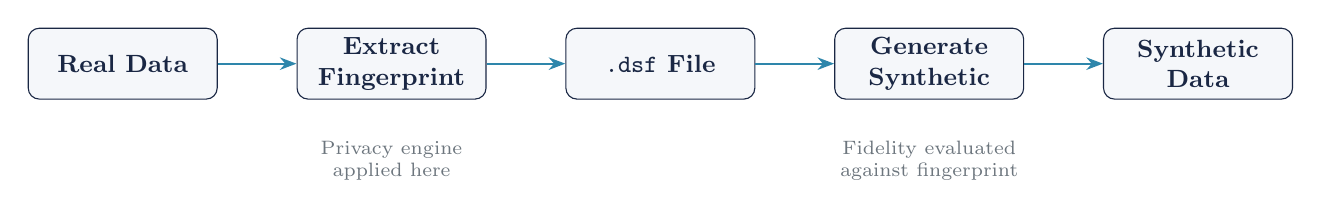
\begin{tikzpicture}[
  node distance=1.0cm,
  box/.style={draw=brand, fill=lightbg, rounded corners=4pt,
              minimum width=2.4cm, minimum height=0.9cm,
              font=\small\bfseries, text=brand, align=center},
  arr/.style={-{Stealth[length=6pt]}, thick, color=accent}
]
  \node[box] (real) {Real Data};
  \node[box, right=of real] (extract) {Extract\\Fingerprint};
  \node[box, right=of extract] (dsf) {\texttt{.dsf} File};
  \node[box, right=of dsf] (generate) {Generate\\Synthetic};
  \node[box, right=of generate] (output) {Synthetic\\Data};

  \draw[arr] (real) -- (extract);
  \draw[arr] (extract) -- (dsf);
  \draw[arr] (dsf) -- (generate);
  \draw[arr] (generate) -- (output);

  \node[below=0.4cm of extract, font=\scriptsize\color{midgray}, align=center]
    {Privacy engine\\applied here};
  \node[below=0.4cm of generate, font=\scriptsize\color{midgray}, align=center]
    {Fidelity evaluated\\against fingerprint};
\end{tikzpicture}
\end{center}

\subsection{Privacy Levels}

\vspace{0.4em}
\noindent
\renewcommand{\arraystretch}{1.2}
\begin{tabularx}{\textwidth}{l c c c X}
\toprule
\textbf{Level} & \textbf{Epsilon ($\varepsilon$)} & \textbf{k-Anon} &
\textbf{Outlier \%} & \textbf{Use Case} \\
\midrule
Minimal  & 5.0  & 3  & 99\% & Low privacy, high utility \\
Standard & 1.0  & 5  & 95\% & Balanced (default) \\
High     & 0.5  & 10 & 90\% & Sensitive environments \\
Maximum  & 0.1  & 20 & 85\% & Maximum privacy guarantees \\
\bottomrule
\end{tabularx}
\renewcommand{\arraystretch}{1.0}

The privacy engine combines differential privacy (Laplace and Gaussian
mechanisms), k-anonymity with rare-value suppression, and outlier
winsorization. A full privacy audit trail records every decision and the
cumulative epsilon budget spent.

\subsection{Federated Fingerprinting \& Certificates}

\textit{New in v0.5.0} --- distributed fingerprint extraction and
cryptographic provenance:

\begin{itemize}[leftmargin=1.4em, itemsep=2pt]
  \item \textbf{Federated Coordinator}: Aggregate fingerprints from
        distributed data sources without centralizing raw data.
  \item \textbf{Synthetic Data Certificates}: \texttt{SyntheticDataCertificate}
        with cryptographic proof of differential privacy guarantees,
        generation metadata, and validation workflow.
  \item \textbf{Pareto Frontier}: Automated exploration of optimal
        privacy--utility trade-offs across epsilon values.
\end{itemize}

\subsection{Formal DP Composition}

\textit{New in v0.5.0} --- advanced privacy accounting beyond naive
$\varepsilon$-summation:

\begin{itemize}[leftmargin=1.4em, itemsep=2pt]
  \item \textbf{R\'{e}nyi DP}: RDP curve tracking at $\alpha$ values 2--128
        with conversion to ($\varepsilon$,$\delta$)-DP.
  \item \textbf{zCDP}: Zero-Concentrated DP with additive $\rho$ composition
        and tighter bounds.
  \item \textbf{Budget Manager}: Global budget tracking across extraction
        runs with composition-aware enforcement.
  \item \textbf{Privacy Evaluation}: Post-generation membership inference
        attack (MIA) testing, linkage attack assessment, and
        NIST SP 800-226 alignment.
\end{itemize}

\subsection{Fidelity Evaluation}

Per-column statistical distance metrics quantify how well synthetic data
matches the source fingerprint:

\vspace{0.4em}
\noindent
\renewcommand{\arraystretch}{1.2}
\begin{tabularx}{\textwidth}{>{\bfseries\color{brand}}l X}
\toprule
\textbf{Metric} & \textbf{Description} \\
\midrule
KS Statistic &
  Kolmogorov-Smirnov two-sample test statistic (sup of CDF difference). \\
Wasserstein-1 &
  Earth Mover's Distance via piecewise-linear inverse CDF integration over
  9 percentile knots. \\
JS Divergence &
  Jensen-Shannon divergence from percentile-bin PMFs, bounded by $\ln 2$. \\
\bottomrule
\end{tabularx}
\renewcommand{\arraystretch}{1.0}

\noindent
Distribution CDFs are computed analytically for Normal, LogNormal, Gamma
(regularized incomplete gamma via Lanczos + Lentz continued fraction),
Pareto, PointMass, and Mixture distributions.

% ══════════════════════════════════════════════════════════════════════════════
\section{Architecture}

\subsection{Layered Crate Architecture}

\begin{center}
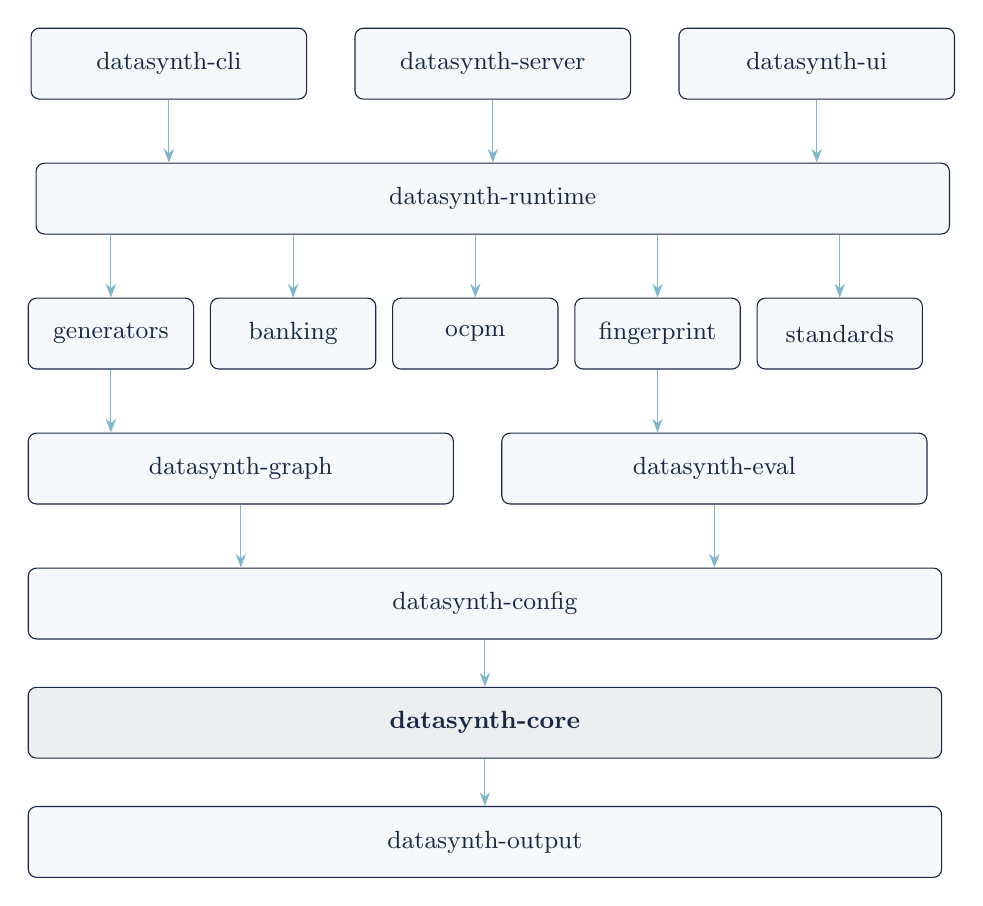
\begin{tikzpicture}[
  node distance=0.5cm,
  layer/.style={draw=brand, fill=lightbg, rounded corners=3pt,
                minimum height=0.9cm, font=\small, text=brand, align=center},
  arr/.style={-{Stealth[length=5pt]}, color=accent!60}
]
  % Top layer
  \node[layer, minimum width=3.5cm] (cli) {datasynth-cli};
  \node[layer, minimum width=3.5cm, right=0.6cm of cli] (server) {datasynth-server};
  \node[layer, minimum width=3.5cm, right=0.6cm of server] (ui) {datasynth-ui};

  % Runtime
  \node[layer, minimum width=11.6cm, below=0.8cm of server] (runtime) {datasynth-runtime};

  % Generator layer
  \node[layer, minimum width=2.1cm, below=0.8cm of runtime.south west,
        anchor=north west, xshift=-0.1cm] (gen) {generators};
  \node[layer, minimum width=2.1cm, right=0.2cm of gen] (bank) {banking};
  \node[layer, minimum width=2.1cm, right=0.2cm of bank] (ocpm) {ocpm};
  \node[layer, minimum width=2.1cm, right=0.2cm of ocpm] (fp) {fingerprint};
  \node[layer, minimum width=2.1cm, right=0.2cm of fp] (std) {standards};

  % Analytics layer
  \node[layer, minimum width=5.4cm, below=0.8cm of gen.south west,
        anchor=north west] (graph) {datasynth-graph};
  \node[layer, minimum width=5.4cm, right=0.6cm of graph] (eval) {datasynth-eval};

  % Config
  \node[layer, minimum width=11.6cm, below=0.8cm of graph.south west,
        anchor=north west] (config) {datasynth-config};

  % Core
  \node[layer, minimum width=11.6cm, below=0.6cm of config, fill=brand!8]
    (core) {\textbf{datasynth-core}};

  % Output
  \node[layer, minimum width=11.6cm, below=0.6cm of core] (output) {datasynth-output};

  % Arrows -- top to runtime (straight down from each)
  \draw[arr] (cli.south) -- (cli.south |- runtime.north);
  \draw[arr] (server.south) -- (runtime.north);
  \draw[arr] (ui.south) -- (ui.south |- runtime.north);

  % Runtime to generators (individual vertical drops)
  \draw[arr] (runtime.south -| gen) -- (gen.north);
  \draw[arr] (runtime.south -| bank) -- (bank.north);
  \draw[arr] (runtime.south -| ocpm) -- (ocpm.north);
  \draw[arr] (runtime.south -| fp) -- (fp.north);
  \draw[arr] (runtime.south -| std) -- (std.north);

  % Generators to analytics
  \draw[arr] (gen.south) -- (gen.south |- graph.north);
  \draw[arr] (fp.south) -- (fp.south |- eval.north);

  % Analytics to config
  \draw[arr] (graph.south) -- (graph.south |- config.north);
  \draw[arr] (eval.south) -- (eval.south |- config.north);

  \draw[arr] (config.south) -- (core.north);
  \draw[arr] (core.south) -- (output.north);
\end{tikzpicture}
\end{center}

\subsection{Production-Grade Infrastructure}

\vspace{0.4em}
\noindent
\renewcommand{\arraystretch}{1.2}
\begin{tabularx}{\textwidth}{>{\bfseries\color{brand}}l X}
\toprule
\textbf{Capability} & \textbf{Details} \\
\midrule
Deterministic Output &
  ChaCha8 PRNG with configurable seed; identical seed $\Rightarrow$ identical
  dataset. \\
Financial Precision &
  \texttt{rust\_decimal} throughout; no IEEE\,754 floating-point artifacts.
  Decimals serialized as strings. \\
Resource Guards &
  Unified CPU, memory, and disk monitoring with automatic throttling and
  graceful degradation (Normal\,$\to$\,Reduced\,$\to$\,Minimal\,$\to$\,Emergency). \\
Collision-Free IDs &
  FNV-1a hash-based UUID factory with generator-type discriminators prevents
  document ID collisions across parallel generators. \\
Streaming Output &
  CSV, JSON, NDJSON, and Apache Parquet (15-column Arrow schema, Zstd
  compression) streaming sinks with backpressure strategies
  (Block, DropOldest, DropNewest, Buffer). \\
API Layer &
  REST + gRPC + WebSocket with Argon2id API-key auth, JWT/OIDC bearer tokens
  (RS256, Keycloak/Auth0/Entra ID), RBAC (Admin/Operator/Viewer),
  sliding-window rate limiting (in-memory or Redis), TLS (rustls),
  async job queue, security headers, and structured audit logging. \\
Desktop UI &
  Tauri + SvelteKit cross-platform application with 15+ configuration pages
  and real-time streaming viewer. \\
Plugin SDK &
  \texttt{GeneratorPlugin}, \texttt{SinkPlugin}, and \texttt{TransformPlugin}
  traits with thread-safe registry for custom extensions. \\
Webhooks &
  Fire-and-forget event dispatch (RunStarted, RunCompleted, RunFailed,
  GateViolation) with HMAC signing and configurable retry. \\
Data Lineage &
  Per-file SHA-256 checksums, \texttt{LineageGraph} tracking
  config$\to$generator$\to$output relationships, W3C PROV-JSON export,
  CLI \texttt{verify} command. \\
Python Wrapper &
  \texttt{datasynth-py} 1.3 with blueprints (sourcing, HR, manufacturing,
  financial reporting, tax, treasury, project accounting, ESG),
  pandas/polars integration, async client, and WebSocket streaming support. \\
\bottomrule
\end{tabularx}
\renewcommand{\arraystretch}{1.0}

% ══════════════════════════════════════════════════════════════════════════════
\newpage
\section{Industry Presets}

DataSynth ships with ten industry-specific configuration presets, each tuned
for realistic business process weightings, chart-of-accounts structures, and
regional multi-company setups.

\vspace{0.4em}
\noindent
\renewcommand{\arraystretch}{1.25}
\begin{tabularx}{\textwidth}{>{\bfseries}l l X}
\toprule
\textbf{Industry} & \textbf{Key Weight} & \textbf{Characteristics} \\
\midrule
Manufacturing       & 40\% P2P & 14 transaction types, multi-level BOM, production routings,
                                  work centers, JIT, quality framework. \\
Retail              & 50\% O2C & 12 transaction types, 7 store types, shrinkage modeling,
                                  loss prevention, markdown patterns. \\
Healthcare          & 15\% H2R & 15 transaction types, payer mix (Medicare/Medicaid/Commercial),
                                  ICD-10/CPT/DRG coding, HIPAA/Stark compliance. \\
Financial Services  & 40\% R2R & Report-heavy, regulatory compliance,
                                  intercompany structures, loan loss provisions. \\
Technology          & 15\% H2R & SaaS revenue recognition, R\&D capitalization,
                                  deferred revenue. \\
Professional Svcs.  & --- & Time-based billing, project accounting, trust accounting. \\
Energy              & --- & Capital-intensive, long-lived assets. \\
Transportation      & --- & Fleet management, route-based costing. \\
Real Estate         & --- & Property portfolios, lease accounting. \\
Telecommunications  & --- & Subscription revenue, network assets. \\
\bottomrule
\end{tabularx}
\renewcommand{\arraystretch}{1.0}

\vspace{0.3em}
\noindent
Each preset supports three complexity tiers:
\textbf{Small} ($\sim$100 GL accounts),
\textbf{Medium} ($\sim$400 accounts), and
\textbf{Large} ($\sim$2\,500 accounts).

% ══════════════════════════════════════════════════════════════════════════════
\section{Statistical Distribution Framework}

DataSynth includes an advanced statistical distribution framework for generating
empirically grounded synthetic data:

\vspace{0.4em}
\noindent
\renewcommand{\arraystretch}{1.2}
\begin{tabularx}{\textwidth}{>{\bfseries\color{brand}}l X}
\toprule
\textbf{Capability} & \textbf{Details} \\
\midrule
Mixture Models &
  Gaussian and Log-Normal mixtures with weighted components (``routine'', ``significant'', ``major'' transactions). \\
Copula Correlation &
  Gaussian, Clayton, Gumbel, Frank, Student-t copulas for cross-field dependencies. \\
Distribution Types &
  Pareto (heavy-tailed), Weibull (time-to-event), Beta (proportions), Zero-inflated (excess zeros). \\
Benford's Law &
  First and second-digit compliance, round number bias, threshold clustering. \\
Regime Changes &
  Economic cycles, acquisition/divestiture effects, recession modeling. \\
Industry Profiles &
  Pre-configured profiles for Retail, Manufacturing, Financial Services. \\
\bottomrule
\end{tabularx}
\renewcommand{\arraystretch}{1.0}

\vspace{0.3em}
\noindent
All distributions include validation tests: Benford's Law MAD, Anderson-Darling
goodness-of-fit, chi-squared, and correlation matrix verification.

% ══════════════════════════════════════════════════════════════════════════════
\section{Use Cases}

\begin{tcolorbox}[keybox={Primary Use Cases}]
\begin{description}[leftmargin=1em, labelwidth=1em, font=\color{brand}\bfseries]
  \item[$\blacktriangleright$] \textbf{Fraud Detection ML} ---
    Train and validate models on labeled fraud typologies with realistic
    base-rate imbalance.

  \item[$\blacktriangleright$] \textbf{Graph Neural Networks} ---
    Export transaction graphs in PyTorch Geometric, Neo4j, DGL, or RustGraph
    format --- including multi-layer hypergraphs --- with pre-computed features
    and train/val/test splits.

  \item[$\blacktriangleright$] \textbf{AML \& KYC Testing} ---
    Generate banking transaction data with structuring, layering, and mule
    patterns for compliance system validation.

  \item[$\blacktriangleright$] \textbf{Audit Analytics} ---
    Produce ISA-compliant audit artifacts and anomaly-injected financial
    data for analytics tool development.

  \item[$\blacktriangleright$] \textbf{ERP Integration Testing} ---
    Generate SAP ACDOCA-format data with full document chains for system
    migration and integration testing.

  \item[$\blacktriangleright$] \textbf{Process Mining} ---
    OCEL\,2.0 event logs for process discovery, conformance checking, and
    variant analysis.

  \item[$\blacktriangleright$] \textbf{SOX \& COSO Compliance Testing} ---
    Internal control definitions with COSO 2013 mappings, SOX 302/404
    certifications, deficiency classification, and SoD conflict detection.

  \item[$\blacktriangleright$] \textbf{Accounting Standards Testing} ---
    Generate revenue contracts (ASC 606/IFRS 15), lease portfolios
    (ASC 842/IFRS 16), fair value measurements, and impairment tests
    with dual-framework reconciliation.

  \item[$\blacktriangleright$] \textbf{Data Quality ML} ---
    Labeled missing values, typos, duplicates, and format variations for
    training data-cleansing models.

  \item[$\blacktriangleright$] \textbf{Drift Detection ML} ---
    Labeled drift events (organizational, process, technology, market, regulatory)
    with magnitude and detection difficulty for drift detection model training.

  \item[$\blacktriangleright$] \textbf{Network Analytics} ---
    Multi-tier vendor networks and customer segmentation graphs with
    relationship strength metrics for supply chain and customer analytics.

  \item[$\blacktriangleright$] \textbf{Causal Inference Testing} ---
    Structural causal models with do-calculus interventions for
    counterfactual scenario generation and what-if analysis.

  \item[$\blacktriangleright$] \textbf{Pipeline Orchestration} ---
    Apache Airflow operators, dbt source generation, MLflow experiment
    tracking, and Spark DataFrame readers for end-to-end ML pipelines.

  \item[$\blacktriangleright$] \textbf{Tax Compliance Testing} ---
    Tax return filing simulation, ASC\,740/IAS\,12 provision computation,
    uncertain tax position modeling, withholding tax treaty benefits.

  \item[$\blacktriangleright$] \textbf{Treasury Operations} ---
    Cash positioning, probability-weighted forecasting, hedge effectiveness
    testing (ASC\,815/IFRS\,9), debt covenant monitoring, and multilateral netting.

  \item[$\blacktriangleright$] \textbf{Project Cost Control} ---
    WBS-based project costing, earned value management (EVM), change order
    tracking, percentage-of-completion revenue recognition, retainage.

  \item[$\blacktriangleright$] \textbf{ESG \& Sustainability Reporting} ---
    GHG Protocol Scope\,1/2/3 emissions, diversity \& pay equity metrics,
    GRI/SASB/TCFD disclosure preparation, supplier ESG assessments.

  \item[$\blacktriangleright$] \textbf{EU AI Act Compliance} ---
    Article 50 synthetic content marking with content credentials and
    Article 10 data governance reports with bias assessments.
\end{description}
\end{tcolorbox}

% ══════════════════════════════════════════════════════════════════════════════
\section{Evaluation \& Auto-Tuning}

DataSynth includes a built-in evaluation framework that measures synthetic
data quality across four dimensions:

\begin{enumerate}[leftmargin=1.4em, itemsep=3pt]
  \item \textbf{Statistical Fidelity} --- KS statistic, Wasserstein-1 (Earth
        Mover's Distance), Jensen-Shannon divergence, Benford's Law MAD,
        Anderson-Darling goodness-of-fit.
  \item \textbf{Coherence} --- Balance-sheet validation, intercompany matching,
        document chain integrity, standards compliance.
  \item \textbf{Data Quality} --- Completeness, consistency, duplicate rates,
        format correctness, uniqueness.
  \item \textbf{ML Readiness} --- Feature distributions, label quality, graph
        structure, train/val/test split balance.
  \item \textbf{Drift Detection} --- Hellinger distance, Population Stability Index (PSI),
        rolling window analysis, detection delay metrics.
\end{enumerate}

\subsection{ML Benchmarks}

Pre-configured benchmarks aligned with ACFE statistics and industry verticals:

\begin{itemize}[leftmargin=1.4em, itemsep=2pt]
  \item \textbf{ACFE-Calibrated}: General fraud (1k), collusion-focused (5k), management override (2k).
  \item \textbf{Industry-Specific}: Manufacturing fraud (5k), retail fraud (10k), healthcare fraud (5k), technology fraud (3k), financial services fraud (5k).
  \item \textbf{Cost-Sensitive}: Asymmetric cost matrices for realistic fraud detection evaluation.
\end{itemize}

\noindent
An \textbf{auto-tuning engine} analyses evaluation results and produces
prioritized configuration patches with expected improvement estimates ---
closing the loop between generation and validation.

\subsection{Quality Gate Engine}

\textit{New in v0.5.0} --- configurable pass/fail thresholds that can block
releases of low-quality synthetic data:

\begin{itemize}[leftmargin=1.4em, itemsep=2pt]
  \item \textbf{8 metrics}: Benford MAD, balance coherence, document chain
        completeness, duplicate rate, missing rate, distribution fit,
        correlation accuracy, anomaly precision.
  \item \textbf{Built-in profiles}: \texttt{strict}, \texttt{default},
        \texttt{lenient} --- or define custom per-metric thresholds.
  \item \textbf{CLI integration}: \texttt{--quality-gate <profile>} with
        exit code 2 on failure for CI/CD pipelines.
\end{itemize}

% ══════════════════════════════════════════════════════════════════════════════
\section{Compliance \& Governance}

\subsection{EU AI Act}

DataSynth implements Article 50 (synthetic content marking) and Article 10
(data governance) requirements:

\begin{itemize}[leftmargin=1.4em, itemsep=2pt]
  \item \textbf{Content Credentials}: \texttt{SyntheticContentMarker} creates
        machine-readable credentials (generator name, version, timestamp,
        config hash) in embedded, sidecar, or both formats.
  \item \textbf{Data Governance Report}: \texttt{DataGovernanceReport} with
        \texttt{BiasAssessment} documenting data provenance, quality metrics,
        and bias evaluation for regulatory submission.
\end{itemize}

\subsection{Regulatory Compliance Documentation}

Pre-built compliance guides with self-assessment templates:

\vspace{0.4em}
\noindent
\renewcommand{\arraystretch}{1.2}
\begin{tabularx}{\textwidth}{>{\bfseries\color{brand}}l X}
\toprule
\textbf{Framework} & \textbf{Coverage} \\
\midrule
EU AI Act & Article 50 content marking, Article 10 governance \\
NIST AI RMF & Self-assessment across MAP, MEASURE, MANAGE, GOVERN \\
GDPR & Article 30 records, DPIA guidance, data minimization \\
SOC 2 Type II & Readiness across 5 Trust Service Criteria \\
ISO 27001:2022 & Annex A alignment (11 implemented, 6 partial) \\
\bottomrule
\end{tabularx}
\renewcommand{\arraystretch}{1.0}

% ══════════════════════════════════════════════════════════════════════════════
\section{DevOps \& Deployment}

\subsection{CI/CD Pipeline}

An 8-job GitHub Actions pipeline ensures release quality:

\begin{enumerate}[leftmargin=1.4em, itemsep=2pt]
  \item \textbf{fmt}: \texttt{cargo fmt --check}
  \item \textbf{clippy}: Lint with \texttt{-D warnings}
  \item \textbf{test}: Cross-platform matrix (Ubuntu, macOS, Windows)
  \item \textbf{eval}: Comprehensive evaluation (23 evaluators, all process families --- main branch only)
  \item \textbf{msrv}: Minimum Supported Rust Version validation (1.88)
  \item \textbf{security}: \texttt{cargo deny} + \texttt{cargo audit}
  \item \textbf{coverage}: \texttt{cargo-llvm-cov} with Codecov
  \item \textbf{benchmarks}: Criterion regression checks on PRs
\end{enumerate}

\subsection{Deployment Options}

\vspace{0.4em}
\noindent
\renewcommand{\arraystretch}{1.2}
\begin{tabularx}{\textwidth}{>{\bfseries\color{brand}}l X}
\toprule
\textbf{Target} & \textbf{Details} \\
\midrule
Docker &
  Multi-stage builds with cargo-chef caching; distroless runtime images
  for server and CLI. \\
Docker Compose &
  Server + Prometheus + Grafana stack with auto-provisioned datasources. \\
Kubernetes &
  Helm chart with HPA (2--10 replicas), PDB, rolling updates, optional
  Redis subchart, Prometheus ServiceMonitor, and ConfigMap/Secret templates. \\
Bare Metal &
  SystemD service with security hardening (NoNewPrivileges, ProtectSystem,
  MemoryMax=4G, CPUQuota=200\%). \\
Release Pipeline &
  Pre-built binaries for 5 platforms, Docker image to GHCR (amd64 + arm64),
  Trivy container scanning. \\
\bottomrule
\end{tabularx}
\renewcommand{\arraystretch}{1.0}

\subsection{Ecosystem Integrations}

Python-native integrations for popular data engineering tools:

\begin{itemize}[leftmargin=1.4em, itemsep=2pt]
  \item \textbf{Apache Airflow}: \texttt{DataSynthOperator}, \texttt{DataSynthSensor},
        and \texttt{DataSynthValidateOperator} for orchestrated generation.
  \item \textbf{dbt}: \texttt{DbtSourceGenerator} for source YAML and seed files.
  \item \textbf{MLflow}: \texttt{DataSynthMlflowTracker} for experiment tracking
        with quality metrics.
  \item \textbf{Apache Spark}: \texttt{DataSynthSparkReader} for direct DataFrame
        loading from DataSynth output.
\end{itemize}

% ══════════════════════════════════════════════════════════════════════════════
\newpage
\section{Getting Started}

\subsection{Quick Start (CLI)}

\begin{tcolorbox}[colback=brand!3, colframe=brand!40, boxrule=0.5pt, arc=3pt,
                   left=8pt, right=8pt, top=6pt, bottom=6pt]
\ttfamily\small
\# Generate with demo preset\\
datasynth-data generate --demo --output ./output\\[6pt]
\# Create an industry-specific config\\
datasynth-data init --industry manufacturing --complexity medium -o config.yaml\\[6pt]
\# Generate from config\\
datasynth-data generate --config config.yaml --output ./output
\end{tcolorbox}

\subsection{Quick Start (Python)}

\begin{tcolorbox}[colback=brand!3, colframe=brand!40, boxrule=0.5pt, arc=3pt,
                   left=8pt, right=8pt, top=6pt, bottom=6pt]
\ttfamily\small
from datasynth\_py import DataSynth\\
from datasynth\_py.config import blueprints\\[6pt]
config = blueprints.retail\_small(companies=4, transactions=10000)\\
synth = DataSynth()\\
result = synth.generate(config=config)
\end{tcolorbox}

\subsection{Server Mode}

\begin{tcolorbox}[colback=brand!3, colframe=brand!40, boxrule=0.5pt, arc=3pt,
                   left=8pt, right=8pt, top=6pt, bottom=6pt]
\ttfamily\small
\# Start REST/gRPC server with 4 worker threads\\
cargo run -p datasynth-server -- --port 3000 --worker-threads 4
\end{tcolorbox}

% ══════════════════════════════════════════════════════════════════════════════
\vspace{1.5em}
\begin{tcolorbox}[keybox={Links \& Resources}]
\renewcommand{\arraystretch}{1.4}
\begin{tabularx}{\textwidth}{>{\bfseries\color{brand}}l X}
  Repository &
    \url{https://github.com/ey-asu-rnd/SyntheticData} \\
  Documentation &
    \url{https://ey-asu-rnd.github.io/SyntheticData/} \\
  Crates.io &
    \url{https://crates.io/crates/datasynth-core} \\
  PyPI &
    \url{https://pypi.org/project/datasynth-py/} \\
\end{tabularx}
\end{tcolorbox}

\vfill
\begin{center}
\textcolor{midgray}{\rule{0.5\textwidth}{0.4pt}}\\[0.8em]
{\small\textcolor{midgray}{%
  DataSynth v0.9.3 \textbullet{}
  Open-source (Apache-2.0) \textbullet{}
  Commercial license available%
}}\\[4pt]
{\small\textcolor{midgray}{%
  \textbf{Contact:} \href{mailto:michael.ivertowski@ch.ey.com}{michael.ivertowski@ch.ey.com}%
}}
\end{center}

\end{document}
